\chapter{Introduction}
\label{chapter:introduction}
\epigraph{So many books, so little time.}{Frank Zappa}

The aim of this work is to ???.

\section{???}
\label{sec:intro-1}
Since at least 1990, there has been exponential growth in the number of academic papers published annually in the biomedical domain~\citep{pautasso2012publication}.  
The number of English language biomedical citations indexed by PubMed\sidenote[][-2cm]{\url{https://www.ncbi.nlm.nih.gov/pubmed}} alone since 1900 have now surpassed 29 million\sidenote[][-1cm]{\url{https://www.ncbi.nlm.nih.gov/pubmed?term=(\%221990\%2F01\%2F01\%22\%5BDate\%20-\%20Publication\%5D\%20\%3A\%20\%223000\%22\%5BDate\%20-\%20Publication\%5D)}}.

\begin{figure}
  \centering
  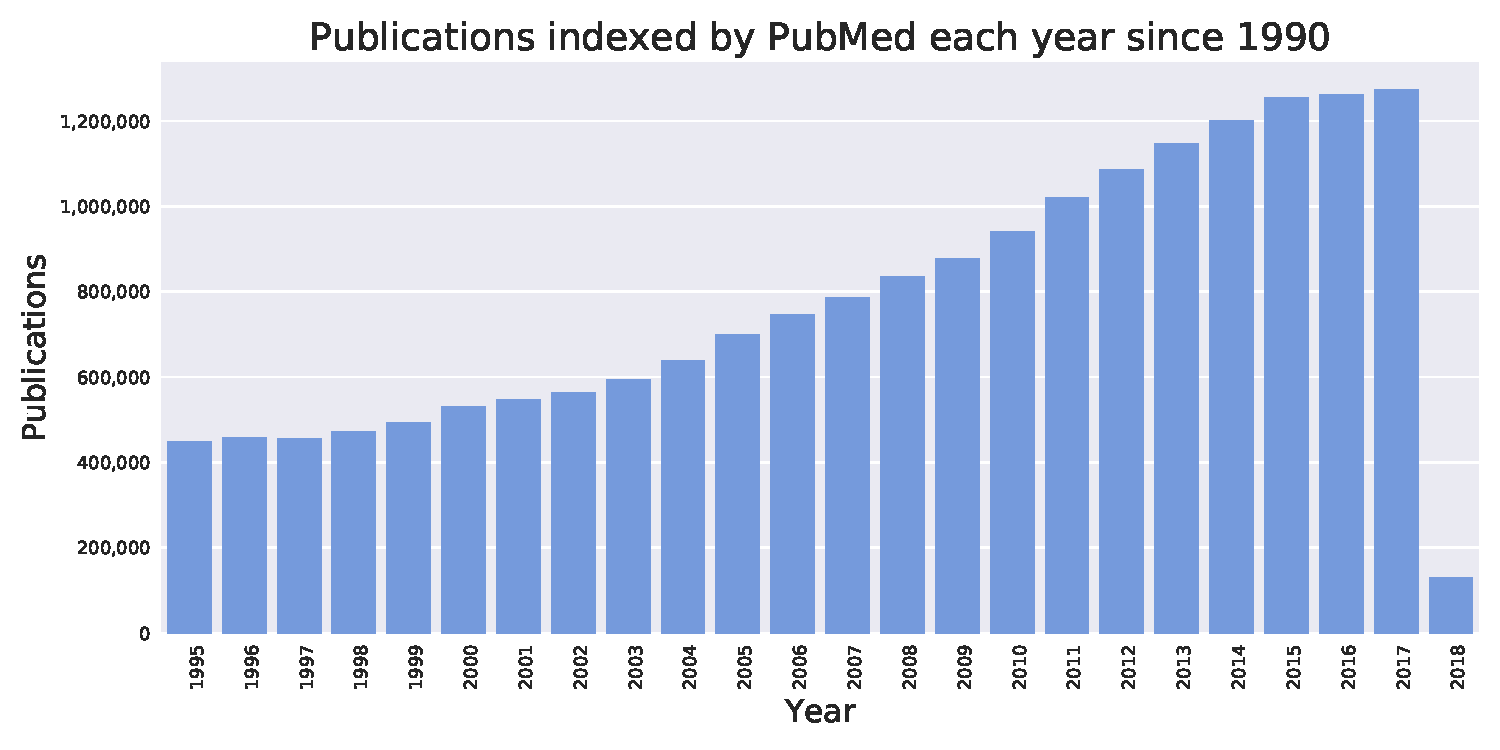
\includegraphics[width=\linewidth]{introduction/pubmed_pub_rate.pdf}
  \caption[][3cm]{According to data indexed by PubMed, biomedical publications remained fewer than 100,000 per year until 1951.  The annual rate began to exceed 1,000,000 in 2011.}
  \label{fig:intro-pubmed-pubs}
\end{figure}

Publications in the domain now exceed 1 million documents per year.  
This poses a serious challenge to researchers needing to understand the state of the field.  
It is effectively impossible for an individual to summarize the larger body of work or even remain abreast of research findings directly relevant to a subtopic.  %\sidenote{Though the severity of the problem has worsened, ~\citet{swanson:1986,swanson1986undiscovered} had already drawn attention to this issue in the 1980s.    
Moreover, how do all of these experimental results interact, and what broader biological context do they define?  
What contradictions exist within the literature?